In recent years, \gls{serverless} computing has emerged as a popular paradigm for building scalable and cost-efficient cloud applications. \Gls{serverless} platforms allow developers to focus on writing code without worrying about server management or infrastructure scaling, while users only pay for the computed time.

While \gls{serverless} computing is an effective model for managing unpredictable and bursty
workloads, it has limitations in supporting latency-critical applications in the IoT, mobile or gaming segments due to cold-start latencies of several hundred milliseconds or more \cite{gackstatter_2022_pushing}. 

An \gls{edge computing} paradigm has emerged to address this issue, which places cloud providers closer to customers to improve latency. However, the issue of cold starts remains a challenge in edge computing. Furthermore, limited CPU power and memory resources in the host environment can further increase latencies, making achieving the desired performance for latency-critical applications difficult.

The underlying issue can be referred to the current runtime environments for \gls{serverless} functions, which primarily rely on \Gls{LXC-Container} technologies like Docker or microVMs like Firecracker. To address these challenges, a more innovative approach would be to execute users' code efficiently and minimize cold start impacts, for instance by replacing heavier containers with lighter alternatives that maintain the advantages of container isolation.

The same requirements for isolation, fast execution and security apply to \gls{WebAssembly} as well. \Gls{WebAssembly} (Wasm) has gained traction as a portable binary format that is executed in an isolated sandbox environment. Wasm is a compilation target, originally designed for browser applications to run e.g. C++ compiled code at near-native speed. This makes WebAssembly the perfect candidate for server-side code execution especially for serverless computing where startup times play a huge role. However, while Wasm was developed with browser execution in mind, standardized system APIs are needed to enable its use on the server side in order to access basic system resources like standard output or file input. Bytecode Alliance is working on the WebAssembly standard and a system interface standard called WASI \cite{webassembly_2023_webassemblywasi}.

\begin{figure}[H]
	\centering
		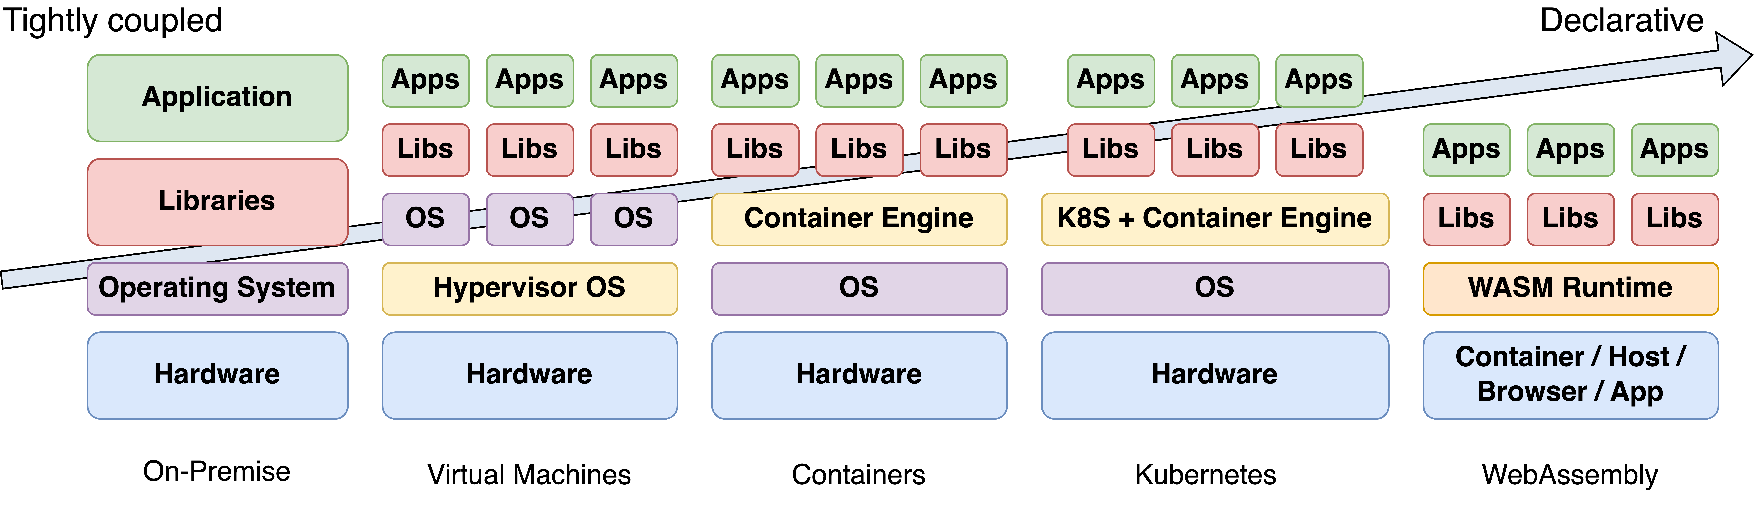
\includegraphics[width=\textwidth,height=\textheight,keepaspectratio]{images/introduction/Cloud_Transformation.pdf}
	\caption{Evolution of computation from on-premise to Wasm based on \cite{randall_2021_wasmcloud}}
	\label{fig:cloud-transformation}
\end{figure}

The figure \ref{fig:cloud-transformation} below depicts the evolution of \gls{cloud computing} from on premise model to the described WebAssembly serverless model.

Another promising browser technology is the usage of V8 \glspl{isolate}. According to Cloudflare, it achieves a startup time faster than a TLS handshake in under five seconds \cite{partovi_2020_eliminating}. The downside of isolates is that they can only execute JavaScript code. This thesis will compare both runtime technologies, but will focus on WebAssembly based runtime technologies.

\section{Research Objectives}
The goal of this research project is to evaluate various factors that affect performance and usability, among other things. Factors such as containerization, selection of WebAssembly runtime, and programming language will be emphasized. Considerations will be made regarding vendor lock-in, and potential strategies for avoiding it will be evaluated. Additionally, the paper will address interesting aspects such as sustainability in terms of resource conservation in the serverless domain. \\
\newline
Based on these requirements, the thesis aims to answer the following research question:
\begin{center}
\textit{"What are the effects of using WebAssembly technology in the serverless domain, particularly concerning the technologies employed (runtime environment, programming language), and how do they compare to existing solutions?"}
\end{center}


\section{Structure of the Thesis}

The remainder of this thesis is organized as follows:
\begin{itemize}
  \item Chapter 2 describes the current state of WebAssembly, including the current specification and any implemented proposals, as well as future proposals. It also covers the WebAssembly System Interface (WASI).
  \item Chapter 3
  \item Chapter 4
  \item Chapter 5
  \item Chapter 6
  \item Chapter 7
  \item Chapter 8
  \item Chapter 9
\end{itemize}